\chapter{系统分析、机制设计与靶场实现}

\section{TripSphere AI 原生应用总体架构}

TripSphere 是一个面向旅行规划、对话修改和订单辅助的 AI 原生应用。它不是单一模型服务，而是由 LangGraph 智能体、工具调用、Java gRPC 微服务、第三方 API、LLM 网关和可观测组件共同构成。本文将其作为应用层故障注入靶场，原因在于它同时包含 Agent 状态机的不确定性和传统分布式系统的失败模式。

从故障传播角度看，TripSphere 可以抽象为五个层次：用户交互层、Agent 编排层、工具与外部服务层、业务微服务层、可观测与实验控制层。用户交互层负责接收 REST 规划请求、CopilotKit 对话请求和 Chat Service 消息；Agent 编排层负责 LangGraph workflow、ReAct 循环以及远程 Order Agent 委托；工具与外部服务层把 Agent 决策转化为地图、景点、酒店、LLM、A2A 和 gRPC 调用；业务微服务层保存行程、商品和订单等领域对象；可观测与实验控制层记录 Trace、Metric、实验编号和故障命中属性。应用层故障注入需要选取这些层之间的语义边界，因为同一个故障可能在 Agent 层表现为错误决策，在工具层表现为 fallback，在服务层表现为 RPC 失败，在可观测层表现为 Trace 断链。

\begin{figure}[htbp]
  \centering
  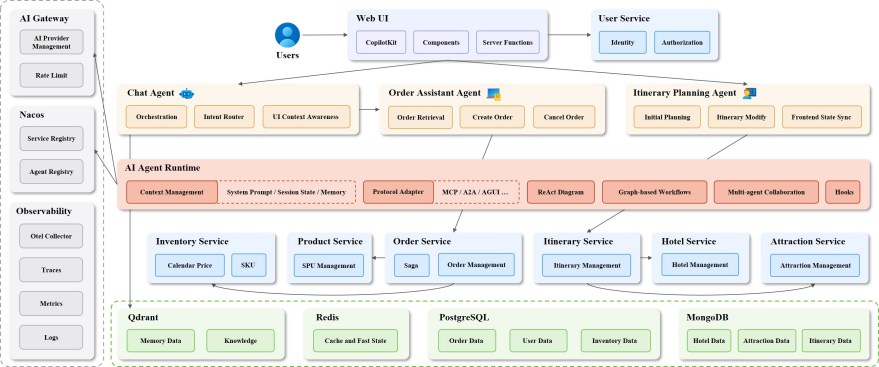
\includegraphics[width=\textwidth]{figures/tripsphere-layered-architecture.png}
  \caption{TripSphere AI 原生应用分层架构}
  \label{fig:tripsphere-layered-architecture}
\end{figure}

表 \ref{tab:ai-native-layers} 进一步给出五层结构中的主要组件、可靠性风险与可观测信号。该分层不是为了重新设计系统，而是为后续故障注入确定边界：本文优先在已有工具包装、RPC client、状态 reducer、路由函数和远程 Agent 调用处插桩，避免大规模改写核心业务。

\begin{table}[htbp]
  \centering
  \small
  \caption{TripSphere AI 原生应用分层结构}
  \label{tab:ai-native-layers}
  \begin{tabularx}{\textwidth}{p{2.6cm}p{3.8cm}XX}
    \toprule
    层次 & 代表组件 & 可靠性风险 & 观测信号 \\
    \midrule
    用户交互层 & REST、CopilotKit、Chat Service & HTTP 成功但业务语义退化 & 状态码、SSE 事件、响应体 \\
    Agent 编排层 & LangGraph workflow、ReAct、Order Agent & 状态丢失、路由错误、远程委托失败 & 节点 Span、状态快照、工具次数 \\
    工具与外部服务层 & 地图、景点、酒店、LLM、A2A & 延迟、异常、响应被篡改 & 工具 Span、Fallback 信号 \\
    业务微服务层 & Itinerary、Product、Order gRPC 服务 & 终态副作用失败、错误码传播 & RPC Span、业务提交率 \\
    可观测与实验控制层 & OpenTelemetry、Tempo、Locust、故障头 & Trace 断链、指标不可关联 & \code{experiment.id}、\code{fault.*} 属性 \\
    \bottomrule
  \end{tabularx}
\end{table}

\section{目标链路与可靠性风险分析}

本文关注三条代表链路，如表 \ref{tab:chains} 所示。链路 A 是 REST 行程规划链，用户提交目的地、日期和偏好后，系统通过 LangGraph workflow 调用地理编码、景点、酒店、LLM 和行程持久化服务，最终产生带数据库副作用的完整行程。链路 B 是 CopilotKit ReAct 对话链，用户围绕已有 itinerary 进行多轮修改，风险集中在状态覆盖、工具选择和条件路由。链路 C 是 Chat 到 A2A 再到 Order 的跨服务链，主聊天 Agent 需要委托远程订单 Agent，再访问商品和订单服务，风险集中在远端 Agent 不可用、Trace 断链和订单草稿状态丢失。

\begin{table}[htbp]
  \centering
  \caption{TripSphere 三条主要链路的结构差异}
  \label{tab:chains}
  \begin{tabularx}{\textwidth}{p{2.5cm}XXX}
    \toprule
    维度 & 链路 A & 链路 B & 链路 C \\
    \midrule
    入口 & REST 规划接口 & CopilotKit 对话入口 & Chat Service 聊天入口 \\
    编排模型 & LangGraph 线性 workflow & LangGraph ReAct 循环 & ADK 根 Agent + A2A 远程 Agent \\
    状态主体 & 单次 PlanningState & MemorySaver checkpoint + itinerary 状态 & ADK Session + 订单草稿内存状态 \\
    终态副作用 & 行程 gRPC 写库 & 前端状态同步为主 & 订单 gRPC 写入 \\
    典型故障 & 工具慢、候选为空、持久化失败 & 状态丢失、路由错误、工具 fallback & 远端 Agent 丢失、A2A 断链、订单草稿丢失 \\
    实验价值 & 验证生成后持久化可靠性 & 验证多轮状态鲁棒性 & 验证跨 Agent 调用完整性 \\
    \bottomrule
  \end{tabularx}
\end{table}

链路 A 的输入输出清晰、端到端副作用明确，并且工具、RPC、LLM 和持久化边界齐全；链路 B 用于验证多轮状态和路由鲁棒性；链路 C 用于验证跨 Agent 调用和跨服务可观测完整性。三者共同覆盖了 AI 原生应用从单次规划、多轮交互到远端委托的主要故障传播路径。

\section{应用层故障模型}

本文将 AI 原生应用层故障定义为发生在 Agent 编排、工具调用、状态读写、模型输出、跨 Agent 通信或业务 RPC 边界上的可观察异常。这类故障不同于资源层故障：它们可能不改变容器、网络或进程状态，却会改变 Agent 看到的数据、走过的路径或最终产生的业务副作用。

表 \ref{tab:fault-model} 给出本文采用的故障分类。该分类不是封闭集合，而是围绕 TripSphere 当前可实验链路整理出的最小可用模型。每一类故障都需要绑定目标、触发条件和观测信号，否则实验者只能说明“系统出错”，无法判断故障是否按声明命中，也无法复现实验。

\begin{longtable}{p{1.5cm}p{2.8cm}p{4.2cm}p{4.2cm}}
  \caption{AI 原生应用层故障分类模型}
  \label{tab:fault-model}\\
  \toprule
  编号 & 类别 & 典型注入点 & 观测重点 \\
  \midrule
  \endfirsthead
  \toprule
  编号 & 类别 & 典型注入点 & 观测重点 \\
  \midrule
  \endhead
  F1 & 工具/RPC 延迟 & 地理编码、景点、酒店、行程持久化、LLM 调用 & 端到端耗时、p95/p99、超时和排队 \\
  F2 & 工具/RPC 异常 & Python 工具函数、gRPC client 调用前 & fallback 是否触发、HTTP 状态码 \\
  F3 & gRPC 错误码 & \code{ItineraryService.CreateItinerary} 等 RPC & 错误分类、502、重试缺口 \\
  F4 & 工具响应篡改 & 景点/酒店列表、地理编码响应、Markdown 文本 & 内容质量、候选数量、下游传播 \\
  F5 & 状态清空/篡改 & \code{itinerary}、\code{pending\_day\_plan}、checkpoint & 状态一致性、前后端同步 \\
  F6 & 路由扰动 & ReAct \code{should\_continue} 条件边 & 是否提前结束、是否错误进入工具 \\
  F7 & 远程 Agent 丢失 & A2A \code{order\_assistant} & 主 Agent fallback、错误提示 \\
  F8 & Trace 断链 & A2A metadata、W3C Trace Context & 实验证据是否完整 \\
  \bottomrule
\end{longtable}

对链路 A 而言，地理编码延迟、候选数据异常和行程持久化失败分别覆盖了“慢但可完成”“内容质量退化”和“终态副作用失败”三类典型现象。对链路 B 而言，状态清空和路由扰动能暴露多轮对话中隐蔽的上下文污染。对链路 C 而言，远程 Agent 丢失和 Trace 断链能验证系统在跨服务调用失败时是否仍保留可解释证据。

\section{故障 DSL 与注入框架}

TripSphere 的故障注入机制围绕低侵入、可配置、请求级隔离、可观测和可回滚五个目标展开。注入逻辑尽量挂载在工具、RPC、LLM、状态 reducer 或路由函数边界，默认关闭时快速早退；故障目标、原语和参数通过环境变量、配置文件或请求头声明；每次实验通过 \code{experiment.id} 隔离；每次故障命中都写入当前 Span；移除请求头或关闭环境变量即可恢复正常路径。

为了让实验者用统一方式声明故障，本文采用请求头 DSL 描述目标、原语和参数，基本形式如下：

\begin{verbatim}
<target>.<primitive>=<arg1>[,<arg2>][,key=value,...]
\end{verbatim}

多条故障通过分号连接。例如：

\begin{verbatim}
tool.geocoding.latency=4000,jitter=200;
rpc.itinerary.create.error=UNAVAILABLE,probability=0.1;
state.itinerary.clear=true
\end{verbatim}

其中 \code{target} 表示注入对象，通常包含组件类型和业务名称；\code{primitive} 表示故障原语；等号右侧表示参数。当前主要原语包括 \code{latency}、\code{exception}、\code{error}、\code{mutate}、\code{clear}、\code{force\_route} 和 \code{drop}。它们分别对应延迟、异常、错误码、响应篡改、状态清空、路由扰动和远程 Agent 不可用等实验维度。

注入框架分为控制面和数据面。控制面读取 \code{FAULT\_INJECTION\_ENABLED}、\code{FAULT\_INJECTION\_SCENARIO}、\code{FAULT\_INJECTION\_FILE}、\code{x-experiment-id} 和 \code{x-fault-scenario}，解析后构造运行时规则。数据面在工具、RPC、LLM、状态 reducer、路由函数或远程 Agent 包装边界执行故障，并把命中结果写入当前 Span。新增注入点时，只需要在已有语义边界加入装饰器或显式调用；新增实验场景时，只需要提供新的 DSL 或配置，不需要改写业务流程。

请求级隔离是该机制的安全基础。每个 HTTP 请求携带自己的实验编号和故障声明，中间件把它们放入异步安全的上下文；后续工具、RPC 和 LLM 节点读取当前请求上下文，而不是读取全局可变变量。对于跨服务链路，实验头进入 gRPC metadata 或 A2A metadata，使不同服务中的 Span 可以按同一个 \code{experiment.id} 聚合。这样既避免误伤其他流量，也让相同 payload、相同故障 DSL 和相同负载条件具备复跑价值。

低侵入插桩优先放在已有观测边界附近，例如 \code{tool\_span}、\code{rpc\_span}、LLM 调用包装函数和状态 reducer。典型方式包括：对工具和 RPC client 在调用前执行 \code{inject\_fault}、返回后执行 \code{maybe\_mutate}；对 reducer 或状态写回点检查 \code{state.*.clear} 规则；对 \code{should\_continue} 等路由函数检查 \code{force\_route}；对 \code{RemoteA2aAgent} 调用边界检查 \code{agent.*.drop} 或 Trace 断链规则。

\section{可观测证据链与安全边界}

一次故障注入实验必须回答三个问题：声明了什么故障，故障是否真的命中，系统如何响应。为此，注入框架需要在当前 Span 上记录 \code{experiment.id}、\code{fault.scenario}、\code{fault.injected}、\code{fault.target}、\code{fault.primitive}、\code{fault.outcome} 和关键参数。实验者可以先按 \code{experiment.id} 找到本次请求或压测窗口，再筛选 \code{fault.injected=true} 验证实际命中。

\begin{verbatim}
{ resource.service.name = "trip-itinerary-planner"
  && .experiment.id = "exp-demo"
  && .fault.injected = true }
\end{verbatim}

有了上述证据，实验者可以把故障声明、工具或 RPC Span、入口耗时、HTTP 状态码、Locust 输出和业务质量指标串联起来。后续若接入 OpenTelemetry spanmetrics connector，还可以把 \code{fault.injected=true}、入口延迟和错误数转为 Prometheus 时间序列，支持 Grafana 看板聚合。

安全边界同样重要。默认状态下，故障注入全局开关关闭，所有注入逻辑应快速早退。启用后，如果配置损坏、字段缺失或 DSL 无法解析，框架不应导致服务启动失败，而应忽略无效规则并保留诊断信息。实验结束后，移除请求级故障头或关闭全局开关即可回到正常路径。对于 LLM 输入输出等可能包含隐私的数据，本文只要求记录故障元数据和必要业务指标，不默认记录完整 prompt、completion 或用户敏感内容。

\section{靶场落地与注入点清单}

TripSphere 当前已经具备可复现应用层故障注入的核心能力。实验者可以通过 \code{x-experiment-id} 标记实验，通过 \code{x-fault-scenario} 声明故障。例如：

\begin{verbatim}
POST /api/v1/itineraries/plannings
x-user-id: 42
x-experiment-id: exp-demo
x-fault-scenario: tool.geocoding.latency=4000
\end{verbatim}

请求进入服务后，实验头被解析为当前请求上下文。当地理编码工具执行时，注入框架检查目标是否匹配；若规则命中，则在真实业务调用前增加约 4000\,ms 延迟，并在当前 Span 上写入 \code{fault.injected=true}、\code{fault.target=tool.geocoding} 和 \code{fault.primitive=latency}。请求返回后，实验者可以通过同一个 \code{experiment.id} 关联 HTTP 响应、Trace 和负载测试输出。

链路 A 已覆盖外部地图 API、候选数据服务、LLM 生成和最终持久化等关键风险点，如表 \ref{tab:chain-a-targets} 所示。这些 target 支持单点归因，也可以通过分号组合形成级联故障。链路 B/C 的状态、路由、远程 Agent 和 A2A Trace 等注入点也复用了同一套 DSL 与上下文传播机制，第四章将基于三条链路的实测数据说明其效果。

\begin{table}[htbp]
  \centering
  \small
  \caption{链路 A 代表性注入点}
  \label{tab:chain-a-targets}
  \resizebox{\textwidth}{!}{%
  \begin{tabular}{lll}
    \toprule
    Target & 语义 & 适用故障 \\
    \midrule
    \code{tool.geocoding} & 高德地理编码 HTTP 调用前 & latency, exception \\
    \code{tool.geocoding.response} & 高德响应返回后 & mutate \\
    \code{rpc.attraction.GetAttractionsNearby} & 景点 gRPC 调用前 & latency, exception, error \\
    \code{tool.attractions.response} & 景点列表返回后 & mutate \\
    \code{rpc.hotel.GetHotelsNearby} & 酒店 gRPC 调用前 & latency, exception, error \\
    \code{tool.hotel.response} & 酒店列表返回后 & mutate \\
    \code{llm.research\_and\_plan.structured} & 结构化 LLM 调用前 & latency, exception \\
    \code{llm.generate\_markdown} & Markdown LLM 调用前 & latency, exception \\
    \code{rpc.itinerary.create} & 行程持久化 gRPC 调用前 & latency, exception, error \\
    \bottomrule
  \end{tabular}}
\end{table}
